\documentclass[tikz, border=10pt]{standalone}
\usepackage{pgfplots}
\usepackage{amsmath}
\usetikzlibrary{backgrounds}
\pgfplotsset{compat=1.18}

\begin{document}
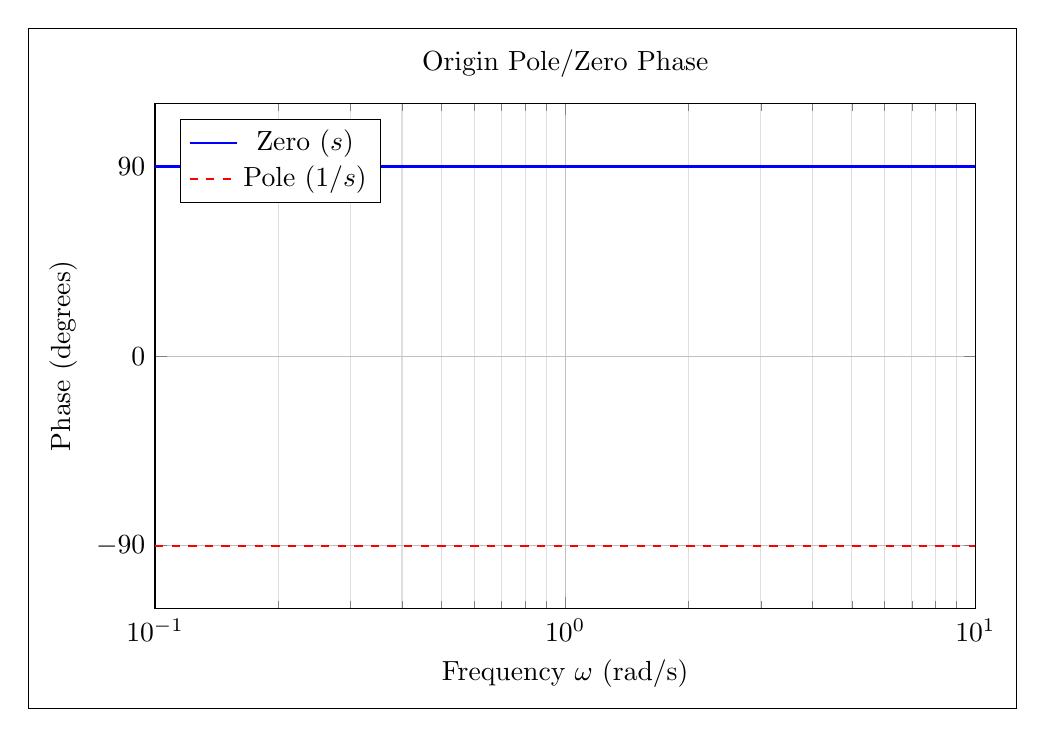
\begin{tikzpicture}[show background rectangle]
    \begin{semilogxaxis}[
        width=12cm, height=8cm,
        title={Origin Pole/Zero Phase},
        xlabel={Frequency $\omega$ (rad/s)},
        ylabel={Phase (degrees)},
        grid=both,
        xmin=0.1, xmax=10,
        ymin=-120, ymax=120,
        minor grid style={gray!25},
        major grid style={gray!50},
        legend pos=north west,
        ytick={-90, 0, 90},
    ]

    % Zero at origin: +90
    \addplot[blue, thick, domain=0.1:10] {90};
    \addlegendentry{Zero ($s$)}

    % Pole at origin: -90
    \addplot[red, dashed, thick, domain=0.1:10] {-90};
    \addlegendentry{Pole ($1/s$)}
    
    \end{semilogxaxis}
\end{tikzpicture}
\end{document}
